\documentclass[12pt]{../manual}
%____________________________________________________________________________
%
%	READ BEFORE USING
%____________________________________________________________________________
%
% This file will not compile unless all the necessary figures are in subfolder named
% "figures" in the same directory as this file. Note that the first time you compile
% this file in a new computer, the references to the figures will all be ???. You
% will have to compile at least three times for all the references to be correct.
% Lastly, take care to not change/remove anything from above this notice. There is
% no guarantee this will compile without all of the definitions and imports above.
%____________________________________________________________________________
%
%	TITLE AND TABLE OF CONTENTS
%____________________________________________________________________________
\begin{document}
\makeheader{Lab 3}{Fall 2019} % Change Semester and Year as needed
\begin{center}
\textbf{\huge ECE 230L - LAB 3}\\~\\
\textbf{\large INTRODUCTION TO CIRCUIT SIMULATION USING PSPICE}\\~\\
\rule{6.5in}{0.5mm}\\
\end{center}

\tableofcontents

\listoffigures

\newpage
%____________________________________________________________________________
%
%	BODY
%____________________________________________________________________________
\section{Objectives of this Laboratory}
The objectives of this laboratory session are to introduce you to the basics of PSpice by learning:
\begin{itemize}
\item How to set-up your PSpice simulation environment,
\item How to represent the circuit elements,
\item How to construct the circuits, and
\item How to simulate the circuits.
\end{itemize}

\section{Setting Up a Circuit Using ORCAD Capture}
To create a circuit in a PSpice environment, one must first launch ORCAD:
\begin{enumerate}
\item Open ORCAD Capture CIS
\item Create a new project by selecting {\bf File} $\to$ {\bf New} $\to$ {\bf Project}
\item Name your project `Lab 3'
\item Choose {\bf Analog or Mixed A/D} under the {\bf Create a New Project Using} menu
\item Select {\bf Create a blank project} when prompted
\end{enumerate}

\begin{myfigure}[label=fig:blankSchematic]{Blank Schematic}{Blank Schematic}
\centering
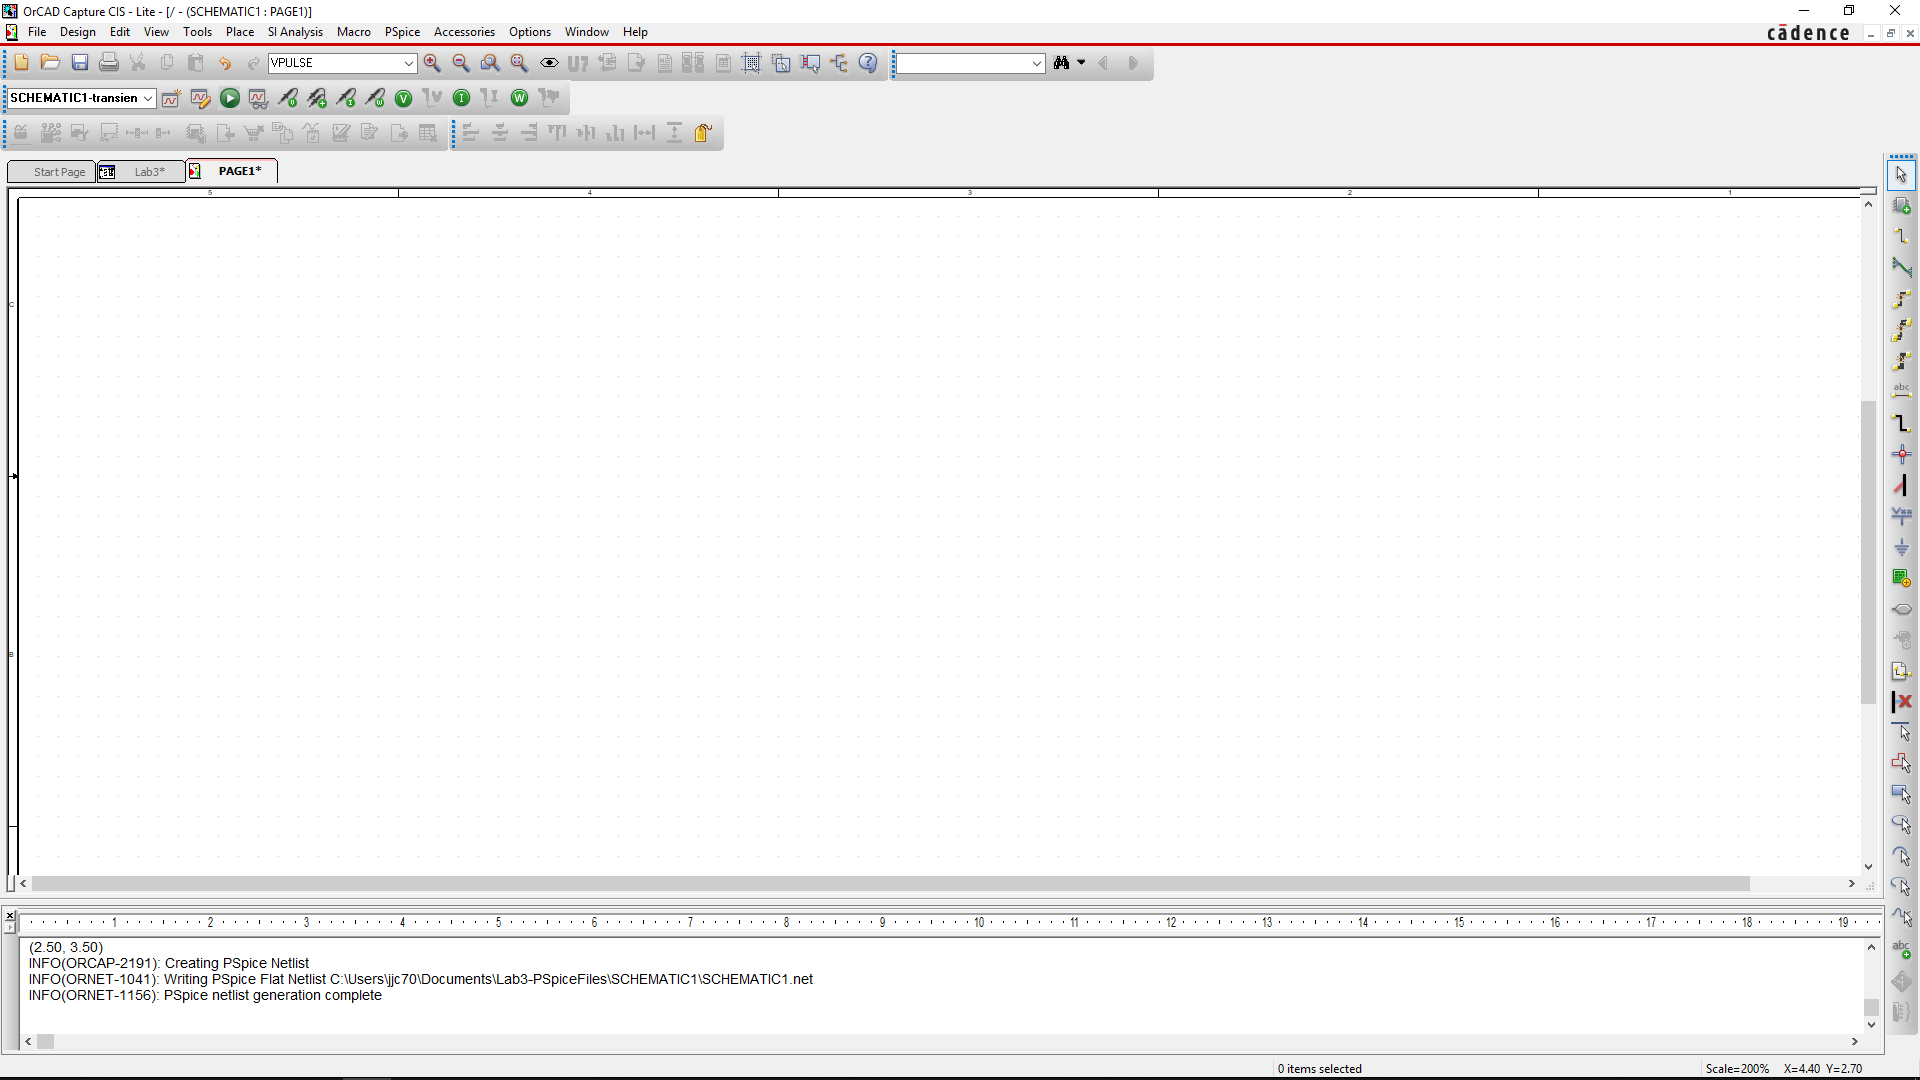
\includegraphics[width=0.9\textwidth]{./figures/BlankSchematic.PNG}
\end{myfigure}

Once the new project has been created, circuit design can begin. Sources, components, ground nodes, and wires can be selected using the {\bf Place} menu.

PSpice will be used to model the circuit in Figure \ref{fig:exampleCircuit} and perform DC, AC, and transient analysis on the circuit.

\begin{myfigure}[label=fig:exampleCircuit]{Example Circuit}{Example Circuit}
\centering
\begin{circuitikz}[scale=2]
\ctikzset{resistors/scale=1.5,batteries/scale=1.5,grounds/scale=1.5,diodes/scale=1.5}
\draw
(0,0) 	to[short] 		++(2,0)
		node[ground] {}
		to[short] 		++(2,0)
		to[C, l_=${C = \SI{1}{\nano\farad}}$]			++(0,2)
		to[short]		++(-2,0)
		to[R, l_=${R_1 = \SI{1}{\kilo\ohm}}$]			++(-2,0)
		to[battery, l_=$v_{in}$]		++(0,-2)
(2,0)	to[R, *-*, l_=${R_2 = \SI{1}{\kilo\ohm}}$]		++(0,2)
;\end{circuitikz}
\end{myfigure}

To make the circuit, 
\begin{enumerate}
\item Add a DC Voltage Source by following \fbox{Place} $\to$ \fbox{PSPice Component} $\to$ \fbox{Source} $\to$ \fbox{Voltage Source} $\to$ \fbox{DC}
\end{enumerate}

Add a DC voltage source to the circuit by following Place $\to$ PSpice Component $\to$ Source $\to$ Voltage Sources $\to$ DC. After adding the voltage source to the schematic, use the Place $\to$ PSpice Components $\to$ Passives menu to insert the remaining resistors and capacitors. Use Ctrl-R to rotate the components. Use Place $\to$ Wire to connect the circuit nodes. To change values of circuit elements, double click on the element and adjust the desired properties. Finally, add a ground node to the circuit schematic. Follow Place $\to$ Ground and select 0/SOURCE as your ground node.

\section{DC Analysis in PSpice}
To perform a DC analysis of the circuit, you will create a new simulation profile. To create a new profile select PSpice $\to$ New Simulation Profile. Name the new profile `dc' and press Create. To analyze the example circuit, select `DC Sweep' in the Analysis Type drop down menu and use the following parameters:
\begin{itemize}
\item Sweep variable > Voltage source: V1
\item Sweep Type: Linear
\item Start Value: 0
\item End Value: 10
\item Increment: 0.01
\end{itemize}
Press `Apply' and `OK' to save the profile settings. Begin the simulation by selecting PSpice-> Run. To view the circuit behavior at a particular point, follow Trace-> Add Trace to select different values to plot or use the voltage and current markers indicated in Figure 1. Plot source voltage, V(R2), I(R1), and I(R2). Figure 3 shows the circuit schematic and figure 4 shows the result of DC analysis (top plot: current, bottom plot: voltage).

\section{AC Analysis in PSpice}

\subsection{Trace Expressions in PSpice}

\section{Transient Analysis in PSpice}

\section{Practice Example}

\section{Exploration: Thevenin Equivalent Circuits}
\subsection{Purpose}
\subsection{Introduction}
\subsection{Exercise}
\subsection{Practice Exercise: Thevenin Equivalent Circuit}

\newpage
\phantomsection % needed in order to link from table of contents to here
\section*{Grading Rubric}
\addcontentsline{toc}{section}{Grading Rubric} % adds section*{} to table of contents
\markboth{Grading Rubric}{Grading Rubric}
\vfill % used to center table vertically on page
\begin{table}[ht!]
\caption{ECE 230L Laboratory 3 Grading Rubric}
\centering
\begin{tabular}{l|c} \hline
Criteria & Points Possible \\ \hline \hline
\textbf{DC Analysis}			& \textbf{10} \\
Circuit Diagram 				& 5 \\
Waveforms 						& 5 \\ \hline
\textbf{AC Analysis}			& \textbf{10} \\
Circuit Diagram 				& 5 \\
Waveforms 						& 5 \\ \hline
\textbf{Transient Analysis}		& \textbf{10} \\
Circuit Diagram 				& 5 \\ 
Waveforms 						& 5 \\ \hline
\textbf{Practice Exercise}		& \textbf{35} \\
Circuit Diagram 				& 5 \\
DC Analysis						& 10 \\
AC Analysis						& 10 \\
Transient Analysis				& 10 \\ \hline
\textbf{Thevenin Equivalent Example Circuit} & \textbf{20} \\
Circuit Diagram					& 10 \\
$V_{OC}$ and $I_{SC}$ Labeled	& 5 \\
Correct $R_{TH}$ Value			& 5 \\ \hline
\textbf{Thevenin Equivalent Challenge Circuit} & \textbf{15} \\
Circuit Diagram					& 5 \\
$V_{OC}$ and $I_{SC}$ Labeled	& 5 \\
Correct $R_{TH}$ Value			& 5 \\ \hline \hline
Total							& 100 \\ \hline
\end{tabular}
\end{table}
\vfill % used to center table vertically on page
\end{document}
